\chapter{Activity Based Computing}

In this chapter we will explain the activity-based paradigm further explained. We will explain why adaptation and awareness is important, and introduce two frameworks that will help us create an activity based client.

\section{Background}
As explained in the introduction, activity based computing is a new computer paradigm that moves focus from application based computer interaction into a higher level computational support for human activities. The paradigm has its outset in clinical work on hospitals, and seeks to aggregate resources to activities, instead of specific applications. An example of such an activity could be the development of our proof of concept. Opening an activity will cause the relevant services and resources to become available to the user, and allow to user to more easily switch between activities and all their associated services and resources. Figure \ref{fig:activitychart} shows an example of the activity "Proof-of-concept development", its associated services and their resources.

\begin{figure}[h!]
  \centering
    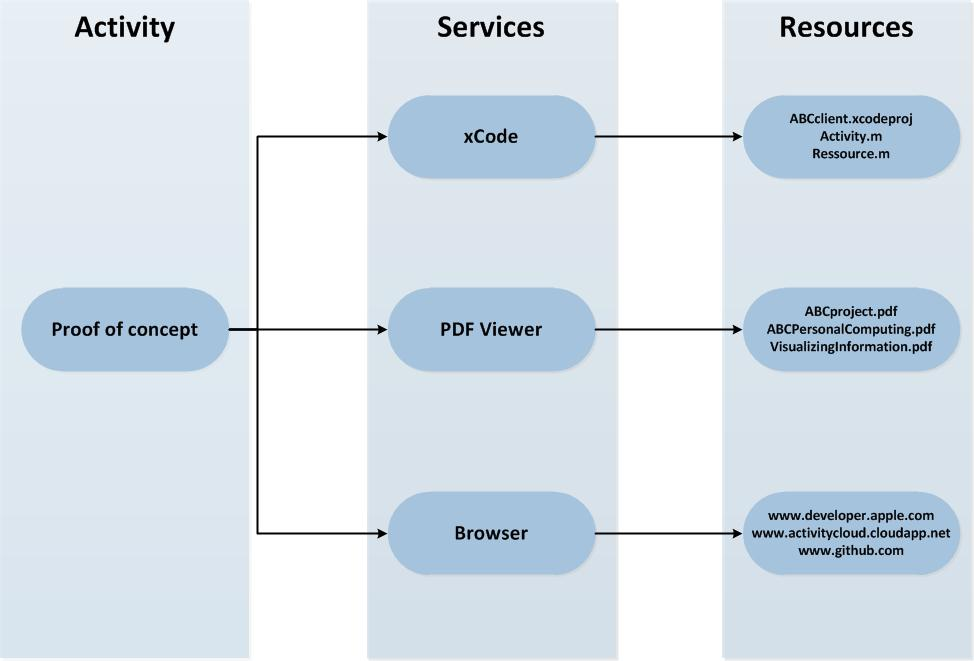
\includegraphics[scale=1.0]{ActivityChart}
  \caption{\emph{The "Proof of Concept" activity. Illustrates how an activity encapsulates its services and resources}}
  \label{fig:activitychart}
\end{figure}

\citet{bardram2011} identifies six principles that forms the basis of the activity based computing paradigm, being; \emph{Activity Centered}, \emph{Activity Suspend and Resume}, \emph{Activity Roaming}, \emph{Acitivty Adaptation}, \emph{Activity Sharing} and \emph{Activity Awareness}. Each of these will be further described in the following.

\begin{description}

	\item[1. Activity Centered] \hfill \\
	An Activity is a computational unit that encapsulates a set of services and their relevant resources. An activity therefore encapsulate digital software and data necessary for a user to carry out their work (activity).
	
	\item[2. Activity Suspend and Resume] \hfill \\
	This allows a user to alternate between several activities and support interruptions that requires the user to perform another task. This is done by suspending the current activity and resuming another.
	
	\item[3. Activity Roaming] \hfill \\
	This principle enables activities to be stored on an infrastructure, like a server, and allows for activities to be suspended on one device, and then resumed on another, to better support user mobility.
	
	\item[4. Activity Adaptation] \hfill \\
	An activity can be displayed and handled on very different devices, and should adapt to the resources available at the resumed devices. In this case resources could be CPU power, screen size and network bandwidth.
	
	\item[5. Activity Sharing] \hfill \\
	Focuses and deals with the collaborative aspect of activities. This principle states that activities are shared among collaborators that appear on a list of participants for any particular activity. If two or more participants engage resumes the same activity they will both be notified and engage in video and audio chat if possible.
		
	\item[6. Activity Awareness] \hfill \\
	Allows for an activity to be context aware, such that it adapts itself to its current environment and work context. This could be to i.e. adapting the user interface or changing activities and services based on where the device is located.

\end{description}

Implementing all of these features enables computational devices to better support human activities, and allow users to move away from the traditional document -and application centered model on a desktop computer. In this thesis we will focus on how to display activities on the iPad and how to adapt the interface to the orientation of the iPad, how to store activities in an infrastructure and how the iPad can be aware of its surroundings. In this chapter we will further explain the principle of adaptation and awareness.

\section{Activity Adaptation and Awareness}
In many work places it is normal for users to carry out their work in several different locations. As an example it would be natural to consider a plausible scenario for a professor during his day at a university:

\begin{quotation}
\emph{
A professor got a day full of meetings at the University. In the beginning of the day he will have a meeting with the head of a study programme at which he teaches a course. They will discuss several course related material, and course goals, and will require the use of the course website, a document with the goals of the study programme, the exercises used in the course. Later he will have a lunch meeting with a fellow colleague in the cantina, to discuss an idea for a project. During preparation he have found several online resources on the matter, and have made a few designs and diagrams he wants to share. After lunch he got a meeting in his office with a couple of students regarding a bachelor thesis, and needs to review some code written, which includes looking over several source code files, as well as a generated documentation file. Afterwards he got a meeting with a PhD student in his office, regarding his thesis that needs review, and also to discuss a certain article found online. During the meeting the search through an article database located online, and find a couple of interesting articles that they save for later use.
}
\end{quotation}

This is a thought scenario but it clearly illustrates two things: first of all there is a need to aggregate resources to certain activities during the day for easy access, and second he only need certain activities at certain locations.

The first issue can be handled by using the activity based paradigm as explained earlier, in order to encapsulate resources with different activities. Now the second issue can be handled by filtering the available activities based on where the user is. Now in this case, only four activities have been mentioned but there might be many more than those. There might be activities planned for the rest of the week, and there might even be activities that are not work related. This could potentially sum up to quite a lot of activities and most of them are only relevant when you are in a specific location.

This is where the principle of activity awareness becomes important. Many wireless technologies exists today, which enables devices to communicate with their surroundings, and using these technologies it would be possible for a device to find out about its current whereabouts.

\begin{figure}[h!]
  \centering
    \includegraphics[scale=0.5]{Moving}
  \caption{\emph{Illustration on how the professor moves between locations in order to carry out his activities}}
  \label{fig:locationmovement}
\end{figure}

With current wireless technologies one could use some kind of antennas in different locations and relate those to certain activities. In this way the device could communicate with these antennas and ask where it is right now and based on the activity relations, only show the activities that takes place in this location. We can specify this kind of filtering as \emph{location filtering}. Location filtering is thus a concrete way of handling activity awareness.

With regards to activity adaptation it is interesting to consider the result of the evaluation from \citet{bardram2009}:
\begin{quotation}
	\emph{
		This means that if an activity is roamed from a display with a large resolution (e.g., 1900×1600) to one with a low resolution (e.g., 800×600), a significant portion of the activity’s application windows will potentially be left outside the visible area of the display. A related issue arose when clinicians asked for activity roaming between very large devices (e.g., the wall display in the team room) to very small devices (e.g., a PDA or a SmartPhone). In principle, the ABC framework can run on a PDA or a Java-enabled SmartPhone using the J2ME edition. The real challenge, however, is to investigate further what it actually means to roam an activity between two such very different types of devices—especially if we take into consideration that the clinicians saw the small devices as tools for more specific actions within the overall activity. One possible approach may be to support roaming a subpart of an activity to a small device, instead of roaming the whole activity.
	}
\end{quotation}

What is really interesting here is that it appears that the same kind of UI is implemented on very different devices, and that a possible solution could be to only handle a subpart of an activity. It should always be discouraged to handle very different devices similarly. It makes sense in standard desktop environments where most computers offer the same screen size and resolution, but when one moves from this environment, as is the case of activity based computing, one should also treat each family of devices differently. This means that PDA's and smartphones should have a distinct UI, tablets should have a distinct UI and so on. One could argue that this would mean a lot of overhead implement different UI's for different devices, but there exist design paradigms that takes this into account, and only require the UI part to changed, and not the rest of the implementation. It is also only natural that the UI is different as these devices would be used very differently as observed in \citet{bardram2009}:

\begin{quotation}
	\emph{
		[\ldots]—especially if we take into consideration that the clinicians saw the small devices as tools for more specific actions within the overall activity
	} 
\end{quotation}

So in order to fully make use of activity adaptation, it is important to recognize that each family of devices is different, and should be treated as such, and that their usage is also different. One would probably not replace a wall display with an iPad and hope to achieve the same thing. This is important to keep in mind when designing the UI of the client on the iPad, in order to support activity adaptation properly.

\section{ABC Framework}
In the following, the infrastructure that will be used to store activities will be described in more detail.
\par\vspace{\baselineskip}
The part of the infrastructure that will be used particularly in this project, is the RESTful API. REST, or representational state transfer, is a web architecture that handles transfer of resource states. A resource can be any meaningful encapsulation of data that allows for a client to make request to a server, when data needs to be changed to a new state. Just like when a user is browsing a website, and everytime a new section of the site is visited the state changes by issuing a request and update the local data according to the response. The data itself will be described using a internet media type. In this case the media type is JSON.

\begin{figure}[!htbp]
  \centering
    \includegraphics[scale=0.8]{architectureCloud}
  \caption{\emph{Illustration of the ABC infrastructure}}
  \label{fig:infrastructure}
\end{figure}

\par\vspace{\baselineskip}
Figure \ref{fig:infrastructure} shows a graphical representation of the RESTful service.
The way the service works is by receiving request from a client through the RESTful service. These requests is then received by \emph{Activity Access} which maps the request to an internal function. That function is called on the \emph{Activity Manager}, which looks at the HTTP header of the initial response, to determine what to do with the JSON data. The JSON data is then mapped to an \emph{Activity} object. Based on this Activity object, an \emph{Activity Wrapper} is produced which is placed in the \emph{Data Table(DT)}, and the activity object itself is serialized and placed as a \emph{Binary Large Object (Blop)}, on the service.

So for example when a GET request is issued by a client, the Activity Manger will lookup the Activity Wrapper in the Data Table, to find out where the Activity object is placed and then deserialize it and map it to JSON data and finally send it back as a response.